\documentclass[12pt,a4paper,notitlepage]{article}

\ifx\pdftexversion\undefined
\usepackage[dvips]{graphicx}
\else
\usepackage[pdftex]{graphicx}
\DeclareGraphicsRule{*}{mps}{*}{}
\fi

\usepackage[colorlinks=false]{hyperref}
\usepackage[T1]{fontenc}
\usepackage[polish]{babel}
\usepackage[utf8]{inputenc}
\usepackage[top=2cm, bottom=2cm, left=2cm, right=2cm]{geometry}
\usepackage{mdwlist}
\usepackage{listings}
\usepackage{cases}

\title{Raport z testów klasy CubicSplineFast}
\author{Piotr Piechal \and
Sławomir Blatkiewicz \and
Michał Zochniak \and
Maciej Daszuta}

\begin{document}

\maketitle

\clearpage

\setcounter{tocdepth}{2}
\tableofcontents

\clearpage

\section{Wstęp}
\subsection{Obiekt testów}
Testom podlegała klasa \emph{CubicSplineFast} z biblioteki matematyczej, której autorem jest dr Thomas Flanagan (www.ucl.ac.uk/~mflanaga/java). Została zaprojektowana tak, by umożliwiać interpolację funkcjami sklejanymi. Proces ten polega na znalezieniu kilku finkcji interpolujących zadany zestaw punktów, a następnie uciągleniu (sklejeniu) ich na styku dziedzin tych funkcji.\\
Skrócony symboliczny opis testowanej klasy:
\begin{verbatim}
public class CubicSplineFast {
	private int nPoints;
	private double[] x;
	private double[] y;
	private double[] d2ydx2;
	private boolean derivCalculated;
	
	public CubicSplineFast(double[] x, double[] y);
	public CubicSplineFast(int nPoints);
	public void resetData(double[] x, double[] y);
	public static CubicSplineFast zero(int n);
	public static CubicSplineFast[] oneDarray(int n, int m);
	public void calcDeriv();
	public double interpolate(double xx);
}
\end{verbatim}
Głównym celem testów jest sprawdzenie poprawności działania funkcji \emph{calcDeriv} oraz \emph{interpolate}. Przetestowane również zostały konstrutkory oraz pozostałe metody pomocnicze z tej klasy.
\textbf{Na potrzeby testowania upubliczniono pola klasy.}

\subsection{Cel}
Naszym celem jest gruntowne przetestowanie tej klasy pod kątem poprawności interpolacji. W tym celu zaprojektowano oraz przeprowadzono zestaw testów czarno- i białoskrzynkowych.

\subsection{Podejście}
W przypadku testów czarnoskrzynkowych, najlepszym sposobem na weryfikację wyników działania funkcji jest zastosowanie \emph{Wyroczni}. Posłużymy się w tej roli środowiskiem Matlab oraz obliczeniami analitycznymi.\\
W przypadku testów białoskrzynkowych będziemy się opierać na analizie kodu funkcji.

\subsection{Wykonane prace}
W ramach projektu wykonano następujące prace:
\begin{itemize*}
\item{Projekt testów i przypadków testowych}
\item{Przeprowadzenie testów}
\item{Analiza wykrytych defektów}
\item{Ocena rezultatów testowania}
\item{Wnioski z testów}
\item{Sporządzenie sprawozdania końcowego}
\end{itemize*}

\subsection{Zasoby}
Działamy w zespole złożonym z czterech studentów, a na przeprowadzenie całego procesu testów przeznaczono okres jednego miesiąca.

\subsection{Podział prac}
Prace podzieliliśmy następująco pomiędzy członków zespołu:
\begin{description}
\item [Piotr Pechal] Kierownik zespołu, złożenie dokumentu sprawozdania, testy czarnoskrzynkowe metod calcDeriv, zero, oneDarray.
\item [Sławomir Blatkiewicz] Testy białoskrzynkowe metody interpolate oraz testy metody resetData.
\item [Michał Zochniak] Testy czarnoskrzynkowe metody interpolate oraz pierwszego konstruktora.
\item [Maciej Daszuta] Testy białoskrzynkowe metody calcDeriv oraz testy drugiego konstruktora.
\end{description}

\subsection{Środowisko}
Testowanie obiektu odbywało się w środowisku NetBeans z wykorzystaniem następującego oprogramowania dodatkowego:
\begin{itemize*}
\item{biblioteka JUnit w wersji 4.8.2 (www.junit.org)}
\item{wtyczka CodeCoverage do środowiska NetBeans.}
\end{itemize*}

\section{Plan testów}

\subsection{CubicSplineFast(double[] x, double[] y)}
\begin{description}
\item [Nazwa testu] ConstructorTest
\item [Dane] Jako dane wejściowe użyte zostaną różne tablice typu double.
\item [Wyniki] Sprawdzane jest, czy wywołanie konstruktora spowoduje pojawienie się odpowiedniego wyjątku lub czy wywołanie konstruktora zakończy się pomyślnie.
\item [Wnioski] Testowanie konstruktora wykazało, że działa on zgodnie z zaleceniami co do użytkownia klasy. Gdy podamy tablice mniejsze niz 2-elementowe lub takie, które mają rózne ilości elementów, konstruktor wyrzuca wyjątek ArrayIndexOutOfBounds.
\end{description}

\vspace*{5mm}
\begin{description}
\item [Opis] Konstruktor ten służy do tworzenia obiektów z użyciem zdefiniowanych wcześniej tablic. Zostało wykonane 5 testów.
 
\item [Sposób realizacji]
\item [Przypadek emptyArray] Próba wywołania konstruktora z pustymi tablicami. Kończy się wyjątkiem ArrayIndexOutOfBounds.

\begin{lstlisting}
@Test (expected = ArrayIndexOutOfBoundsException.class)
public void emptyArray() {
    double[] x = new double[] { };
    double[] y = new double[] { };
    CubicSplineFast csf = new CubicSplineFast(x, y);
}
\end{lstlisting}

\item [Przypadek oneElementArray] Próba wywołania konstruktora z tablicami jednoelementowymi. Kończy się wyjątkiem ArrayIndexOutOfBounds.

\begin{lstlisting}
@Test (expected = ArrayIndexOutOfBoundsException.class)
public void oneElementArray() {
    double[] x = new double[] { 1 };
    double[] y = new double[] { 2 };
    CubicSplineFast csf = new CubicSplineFast(x, y);
}
\end{lstlisting}

\item [Przypadek twoElementArray] Próba wywołania konstruktora z tablicami dwuelementowymi. Konstruktor nie zwraca błędu. Sprawdzane jest, czy dane tablice rzeczywiście zostały ustawione.

\begin{lstlisting}
@Test
public void twoElementArray() {
    double[] x = new double[] { 1, 3 };
    double[] y = new double[] { 2, 1 };
    CubicSplineFast csf = new CubicSplineFast(x, y);
    assertArrayEquals(x, csf.x, eps);
    assertArrayEquals(y, csf.y, eps);
}
\end{lstlisting}

\item [Przypadek normalArray] Próba wywołania konstruktora z tablicą 5-elementową. Konstruktor nie zwraca błędu. Sprawdzane jest, czy dane tablice rzeczywiście zostały ustawione.

\begin{lstlisting}
@Test
public void normalArray() {
    double[] x = new double[] { 1, 2, 3, 4, 5 };
    double[] y = new double[] { 2, 1, 2, 1, 0 };
    CubicSplineFast csf = new CubicSplineFast(x, y);
    assertArrayEquals(x, csf.x, eps);
    assertArrayEquals(y, csf.y, eps);
}
\end{lstlisting}

\item [Przypadek differenyArrays] Próba wywołania konstruktora z tablicami, które różnią się ilością elementów. Kończy się wyjątkiem ArrayIndexOutOfBounds.

\begin{lstlisting}
@Test (expected = ArrayIndexOutOfBoundsException.class)
public void differenyArrays() {
    double[] x = new double[] { 1, 2, 3, 4 };
    double[] y = new double[] { 2, 1, 3 };
    CubicSplineFast csf = new CubicSplineFast(x, y);
}
\end{lstlisting}

\end{description}

\subsection{CubicSplineFast(int nPoints)}
\begin{description}
\item [Nazwa testu] IntConstructorTest
\item [Dane] Jako dane wejściowe użyte zostaną różne wartości liczbowe typu int (wartości dodatnie, ujemne, 0)
\item [Wyniki] Sprawdzana jest wartość obiektu utworzonego przez konstruktor (czy jest różna od null), zaś w przypadku niektórych testów spodziewane jest wywołanie wyjątku NegativeArraySizeException (nie da się utworzyć tablicy o ujemnym rozmiarze, a w/w konstruktor tworzy tablice o rozmiarach zgodnych z podanymi wartościami liczbowymi).
\item [Związki] Najpierw zadeklarowane są obiekty klasy CubicSpineFast. Następnie jest sprawdzane (przed użyciem konstruktora), czy ich wartość wynosi null. Następnie wywoływany jest konstruktor z różnymi wartościami liczbowymi. Test ten potwierdza, że to konstruktor utworzył obiekty.
\item [Wnioski] Podczas testowania konstruktora okazało się, że w przypadku, gdy jako wartość liczbową podamy 0 tworzona jest tablica o takim rozmiarze. W wypadku podania wartości dodatniej dzieje się to samo. Natomiast jeżeli podamy wartość ujemną, program wywołuje wyjątek NegativeArraySizeException i tablica nie zostaje utworzona.
\end{description}
\vspace*{5mm}
\begin{description}
\item [Opis] Kontruktor ten służy do tworzenia obiektów zawierających tablice z zerowymi wartościami x i y.
Przede wszystkim sprawdzana jest liczba punktów zapisanych do wew. tablic obiektu. Zostały napisane 3 testy.
 
\item [Sposób realizacji]
\item [Przypadek secondConstructor\_Test] Jest to normalny przypadek tworzenia obiektu z tablicami wew. o rozmiarze 0. Sprawdzana jest prawdziwość relacji równości liczby punktów 0 z nowo zapisaną liczbą punktów.

\begin{lstlisting}
@Test
public void secondConstructor_Test(){
    cs = new CubicSplineFast(0);
    assertEquals(0, cs.nPoints);
}
\end{lstlisting}

\item [Przypadek secondConstructor\_Test2] Sprawdzana jest równość długości tablicy wewnętrznej przechowującej węzły z liczbą węzłów przechowywaną również wewnętrznie.

\begin{lstlisting}
@Test
public void secondConstructor_Test2(){
    cs = new CubicSplineFast(10);
    assertEquals(cs.x.length, cs.nPoints);
}
\end{lstlisting}

\item [Przypadek secondConstructor\_Test3] Sprawdzana jest równość tablic wewnętrznych przechowujących węzły i wartości funkcji dla tych węzłów, po utworzeniu wyzerowanych tablic.

\begin{lstlisting}
@Test
public void secondConstructor_Test3(){
	cs = new CubicSplineFast(10);
	for(int i=0; i<cs.nPoints; i++){
	    assertEquals(cs.x[i], cs.y[i], eps);
	}
}
\end{lstlisting}

\item [Wynik] Konstruktor prawidłowo tworzy obiekt CubicSplineFast o wyzerowanych elementach tablic przechowującej wartości x i y na podstawie podanej liczby węzłów.
\end{description}
\subsection{resetData(double[] x, double[] y)}
\begin{description}
\item [Opis] Została przetestowana metoda resetData przy pomocy dwóch przypadków testowych: resetData\_Test i resetData\_Test2.
Metoda resetData ma za zadanie zastąpić wewnętrzne tablice nowymi tablicami wartości podanymi jako parametry.
\item [Sposób realizacji]
\item [Przypadek resetData\_Test] Sprawdzane dla tablic 3-elementowych. Tablice mają równe długości, czyli jest to normalny przypadek testowy. Sprawdzana jest w pętli prawdziwość równości elementów wewnętrznej tablicy z elementami tablic, które były przekazane testowanej metodzie, w celu uzasadnienia czy elementy tablic-parametrów prawidłowo się zapisały w tablicach przechowywanych przez obiekt CubicSplineFast.

\begin{lstlisting}
@Test
public void resetData_Test(){
    double[] expected_x = new double[]{1, 2, 3};
    double[] expected_y = new double[]{1, 2, 3};
    cs = new CubicSplineFast(3);

    cs.resetData(expected_x, expected_y);
    for(int i=0; i<cs.nPoints; i++){
        assertEquals(expected_x[i], cs.x[i], eps);
    }
    for(int i=0; i<cs.nPoints; i++){
        assertEquals(expected_y[i], cs.y[i], eps);
    }
}
\end{lstlisting}

\item [Przypadek resetData\_Test2] Parametrami badanej metody są tablice równej długości. Natomiast tworzony jest obiekt CubicSplineFast o wew. tablicach długości większej od długości parametrów. Dzięki temu po wywołaniu testowanej metody, długość wewnętrznych tablic jest ustawiane na długość parametrów(czyli są skracane, a liczba punktów dalej jest taka sama). To powoduje że przy ustawianiu elementów wew. tablic nastąpi
wystąpienie wyjątku o indeksie tablicy wykraczającym poza tablicę.

\begin{lstlisting}
@Test(expected=ArrayIndexOutOfBoundsException.class)
public void resetData_Test2(){
    double[] expected_x = new double[]{1, 2, 3};
    double[] expected_y = new double[]{1, 2, 3};
    cs = new CubicSplineFast(10);

    cs.resetData(expected_x, expected_y);
    for(int i=0; i<cs.nPoints; i++){
        assertEquals(expected_x[i], cs.x[i], eps);
    }
    for(int i=0; i<cs.nPoints; i++){
        assertEquals(expected_y[i], cs.y[i], eps);
    }
}
\end{lstlisting}

\item [Wyniki] Metoda prawidłowo zapisuje tablice pod warunkiem że parametrami są tablice o takiej samej długości jak tablice wewnętrzne dotychczasowe.
\end{description}
\vspace*{5mm}
\begin{description}
\item [Opis] Przetestowane zostały 3 przypadki pokrycia instrukcji metody calcDeriv. Służy ona do obliczenia drugich pochodnych potrzebnych przy algorytmie interpolacji funkcjami sklejanymi.

\item [Sposób realizacji]

\item [Przypadek calcDeriv\_WithOnePointTest] W związku z tym że testowana metoda jest wywoływana tylko w konstruktorze należało nałożyć warunki wejściowe dla metody przy pomocy pierwszego konstruktora. Tworzony jest obiekt z tablicami 1-elementowymi. Dzięki temu nie zostanie pokryte wnętrze pętli for i dalsze instrukcje za nią, z tego powodu że utworzona liczba punktów jest zbyt mała aby przeprowadzić obliczenie pochodnych. Z tego względu wyrzucany jest wyjątek ArrayIndexOutOfBoundsException.
Pokrycie instrukcji w metodzie dla tego przypadku wynosi 28%.

\begin{lstlisting}
@Test(expected=ArrayIndexOutOfBoundsException.class)
public void calcDeriv_WithOnePointTest() {
    double[] x3 = new double[]{1};
    double[] y3 = new double[]{4};
    cs = new CubicSplineFast(x3, y3);
}
\end{lstlisting}

\item [Przypadek calcDeriv\_WithTwoPointsTest] Tworzony jest obiekt z tablicami wewn. 2-elementowymi przy pomocy pierwszego kontruktora. Liczba elementów 2 powoduje że tylko wnętrze pętli for nie jest pokrywane, ponieważ potrzebna jest liczba węzłów >= 3.
Pokrycie instrukcji wynosi 64%.

\begin{lstlisting}
@Test
public void calcDeriv_WithTwoPointsTest() {
    double[] x3 = new double[]{1, 3};
    double[] y3 = new double[]{4, 5};
    cs = new CubicSplineFast(x3, y3);
}
\end{lstlisting}

\item [Przypadek calcDeriv\_WithThreePointsTest] Tworzony jest obiekt z tablicami 3-elementowymi, czyli z minimalną liczbą węzłów aby pokryć całość metody, również pętlę for.
Pokrycie instrukcji wynosi 100%.

\begin{lstlisting}
@Test
public void calcDeriv_WithThreePointsTest() {
    double[] x3 = new double[]{1, 3, 5};
    double[] y3 = new double[]{4, 5, 6};
    cs = new CubicSplineFast(x3, y3);
}
\end{lstlisting}

\item [Wynik] Pokrycie pełne następuje przy podaniu obu tablic co najmniej 3-elementowych.
\end{description}



\subsection{zero(int n)}
\begin{description}
\item [Nazwa testu] testZero1
\item [Dane] Sprawdzony jest przypadek podania długości wektora danych mniejszej od 3
\item [Wyniki] Sprawdzano czy funkcja zwraca wyjątek przewidziany przez twórcę w takiej sytuacji
\item [Wnioski] Nie stwierdzono żadnych nieprawidłowych zachowań
\end{description}
\vspace*{5mm}
\begin{description}
\item [Nazwa testu] testZero2
\item [Dane] Sprawdzony jest przypadek podania poprawnej długości wektora danych
\item [Wyniki] Sprawdzano czy funkcja prawidłowo ustala wielkości wektorów będących polami klasy oraz czy są one zerowane, a także czy w tym przypadku funkcja nie zwróci nieouzasadnionego wyjątku
\item [Wnioski] Nie stwierdzono żadnych nieprawidłowych zachowań
\end{description}
\subsection{oneDarray(int n, int m)}
\begin{description}
\item [Nazwa testu] testOneDarray1
\item [Dane] Sprawdzony jest przypadek podania zerowej długości wektora danych.
\item [Wyniki] Funkcja utworzyla tablicę o zerowej długości.
\item [Wnioski] Funkcja powinna zwracać wyjątek o zerowej długości tablicy by poinformować użytkownika, że prawdopodobnie przekazał jej złe dane.
\end{description}
\vspace*{5mm}
\begin{description}
\item [Nazwa testu] testOneDarray2
\item [Dane] Sprawdzony jest przypadek podania poprawnej długości wektora danych oraz rozmiaru tablicy.
\item [Wyniki] Funkcja tworzyła wektory i tablice o poprawnych wymiarach.
\item [Wnioski] Nie stwierdzono żadnych nieprawidłowych zachowań.
\end{description}
\subsection{calcDeriv()}
\subsubsection{Testy czarnoskrzynkowe}
\textbf{Wyrocznią były obliczenia algebraiczne drugiej pochodnej funkcji matematycznych i podstawienie do jej wzoru wybranych punktów danych.}
\begin{description}
\item [Nazwa testu] testCalcDeriv1
\item [Dane] Sprawdzony jest przypadek podania funkcji okresowej sinus.
\item [Wyniki] Wyniki zwrócone przez funkcję były obarczone błędem ok 0.3 w stosunku do wyników Wyroczni.
\item [Wnioski] Taki bład może wynikać z błędów zaokrągleń lub niedokładności użytej metody numerycznej. 
\end{description}
\vspace*{5mm}
\begin{description}
\item [Nazwa testu] testCalcDeriv2
\item [Dane] Sprawdzony jest przypadek podania funkcji stałej.
\item [Wyniki] Wyniki zwrócone przez funkcję były porpawne.
\item [Wnioski] Nie stwierdzono żadnych nieprawidłowych zachowań.
\end{description}
\vspace*{5mm}
\begin{description}
\item [Nazwa testu] testCalcDeriv3
\item [Dane] Sprawdzony jest przypadek podania funkcji $x^{-3}$.
\item [Wyniki] Wyniki zwrócone przez funkcję były całkowicie niepoprawne. Druga pochodna w badanym przedziale powinna być stale ujemna, natomiast funkcja zwróciła wartości oscylujące zupełnie niezgodne pod względem wartości z wynikami Wyroczni.
\item [Wnioski] Zastosowany algorytm jest niestabilny lub posiada błędy.
\end{description}
\subsubsection{Testy białoskrzynkowe}
\begin{description}
\item [Nazwa testu] TestCalcDeriv
\item [Dane] Tablice x i y, w których zawarte są współrzędne kolejnych punktów funkcji, której drugiej pochodnej szukamy. Dane te to liczby typu double, zarówno dodatnie, ujemne jak i 0. Ponadto sprawdzane jest, jak ilość wskazanych punktów działa na wykonywanie metody.
\item [Wyniki] metoda nie zwraca żadnej wartości, jednak sprawdzane są wyjątki, które wystąpiły podczas wykonywania testów oraz różne ścieżki wykonania tej metody.
\item [Związki] Przy testowaniu tej metody nie jest ona wywoływana bezpośrednio. W przypadkach testowych wywoływany jest konstruktor tworzący tablice współrzędnych punktów i to on wywołuje metodę calcDeriv() z określonymi punktami.
\item [Wnioski] Podczas testowania metody TestCalcDeriv sprawdzono 11 różnych zestawów współrzędnych x i y. Celem niektórych z tych zestawów było wywołanie wyjątku ArrayIndexOutOfBoundsException, który ujawniał się w kilku przypadkach:
\begin{itemize*}
\item{współrzędnych x było więcej niż y}
\item{współrzędnych x było mniej niż 2}
\item{współrzędnych x i y było mniejszej niż 2}
\item{współrzędnych y nie było wcale.}
\end{itemize*}
Wystąpienie tego wyjątku wynikało to z faktu, że w metodzie używane są trzy różne współrzędne: i-1, i oraz i+1.\\
W przypadku, gdy liczba współrzędnych była równa 2, pętle for obecne w metodzie nie były uruchamiane (wynika to z warunków tych pętli).\\
Dla ilości współrzędnych większej niż 2 metoda działa poprawnie. Zarówno dla wartości ujemnych, 0 i wartości dodatnich. Podobnie dla ułamkowej deklaracji liczby (np. 1/3). W przypadku, gdy ilość współrzędnych y była większa niż x metoda również działa poprawnie, pomijając współrzędne y, które nie mają swoich odpowiedników w tabeli x.\\
Metodzie calcDeriv brakuje obsługi błędów oraz informowania użytkownika o błędnych danych wyjściowych (np. niewystarczającej ilości współrzędnych). 
\end{description}
\subsection{interpolate(double xx)}
\subsubsection{Testy czarnoskrzynkowe}
\begin{description}
\item Testy interpolacji w węzłach
\item [Nazwa testu] KnotTestParameter
\item [Opis] Została napisana klasa testowa za pomocą JUnit służąca do testowania własności $S(x_i) = f(x_i)$ gdzie $S$ to funkcja interpolująca, $f$ to funkcja wzorcowa a $x_i$ to zadany węzęł.
\item [Sposób realizacji] Klasa testowa jest zbudowana przy pomocy testu parametryzowanego. Zostają zadane różne zestawy danych testowych, składających się z funkcji wzorcowej postaci: tablice double x zawierająca węzły oraz tablica double y zawierająca wartości funkcji wzorcowej w węzłach. Następnie dla każdego zestawu sprawdzane jest, czy wynik interpolacji w węźle $x[i]$ jest równy wartości funkcji wzorcowej $y[i]$
\begin{lstlisting}
class KnotTestParameter
{
    public KnotTestParameter(double[] x, double[] y)
    {
        this.x = x;
        this.y = y;
    }

    public double[] x;
    public double[] y;
}

@RunWith(value = Parameterized.class)
public class KnotTest
{
    KnotTestParameter param;

    public KnotTest(KnotTestParameter param)
    {
        this.param = param;
    }

    @Parameters
    public static Collection<Object[]> params()
    {
       	/* ... */
    }

    @Test
    public void testKnot()
    {
        CubicSplineFast spline = new CubicSplineFast(param.x, param.y);
        for(int i = 0; i < param.x.length; i++)
        {
            assertEquals(param.y[i], spline.interpolate(param.x[i]), EPS);
        }
    }

}
\end{lstlisting}
Oczekujemy tego, że w węzłach wartości funkcji interpolującej będą takie same jak wartości funkcji wzorcowej. Trzeba wziąć pod uwagę ewentualne błędy precyzji/zaokrągleń.
\item [Wyniki] Udało się zmusić klasę do wygenerowania błędnego wyniku (powyżej dopuszczalnego błędu precyzji).
\end{description}
\vspace*{5mm}
\begin{description}
\item [Testy interpolacji z wyrocznią]
\item [Opis] Klasa została przetestowana pod kątem zgodności z inną implementacją interpolacji za pomocą funkcji sklejanych. Jako wyrocznia został wybrany program \textbf{Matlab 7.12.0}.
\item [Sposób realizacji] Została stworzona klasa w Javie do generowania danych do Matlaba. Klasa dostaje funkcję wzorcową (węzły oraz wartości węzłów) oraz argumenty dla których ma być dokonana interpolacja. Następnie dokonywana jest interpolacja dla tych argumentów a jej wynik zapisywany. Tworzony jest zestaw danych do Matlaba:
\begin{lstlisting}
knownX = [-2.0, ... 2.0]; % wezly
knownY = [-0.9092, ... 0.9092]; % wartosci funkcji w wezlach
intX = [-0.5, ... -0.2]; % argumenty do interpolacji
intY = [-0.4794, ... 0.3894]; % wyniki interpolacji CubicSplineFast
\end{lstlisting}
Następnie dla danych testowych wywoływany jest skrypt w Matlabie który dokonuje interpolacji za pomocą funkcji spline. Następnie interpolacja Matlabem jest porównywana do interpolacji CubicSplineFast. Sprawdzana jest również monotoniczność otrzymanej funkcji.
\begin{lstlisting}
matlabY = spline(knownX, knownY, intX);
diff = intY - matlabY;
disp(['Largest error: ' num2str(max(abs(diff)))]);
for i = 2:length(intX)
    diffInt = intY(i) - intY(i-1);
    diffMat = matlabY(i) - matlabY(i-1);
    if(sign(diffInt) ~= sign(diffMat))
        disp(['Monotony fail: ' num2str(i) ' int: ' num2str(diffInt) ' matlab: ' num2str(diffMat)])
    end
end
\end{lstlisting}
Oczekujemy tego, że wyniki interpolacji będą mniej lub bardziej się pokrywać i będą miały taki sam kształt. Trzeba wziąć pod uwagę błędy precyzji oraz to, że Matlab prawdopodobnie implementuje inny (lepszy?) algorytm interpolacji funkcjami sklejanymi.
\item [Wyniki] We wszystkich przypadkach testowych obserwujemy mniejsze lub większe odchylenia interpolacji Matlabowej od interpolacji CubicSplineFast. Każdy testowany przypadek przeszedł ``test monotoniczności'' czyli można uznać że otrzymywane krzywe miały taki sam kształt.\\

Wykonane zostały testy na następujących funkcjach:

Funkcja $f(x) = 5$

Węzły $x = [0:1:10]$

Interpolowana w punktach $x = [0:0.01:10]$

Wynik klasy pokrywa się (nie licząc błędów precyzji rzędu $10^{-16}$) z wynikiem otrzymanym w Matlabie.

Funkcja $S(x) = $
%	3 & $x = 0$\\
%	8 & x = 1\\
%	7 & x = 2\\
%	8 & x = 3\\
%	5 & x = 4\\
%	3 & x = 5\\
%	5 & x = 6\\
%	5 & x = 7\\
%	6 & x = 8\\
%	1 & x = 9\\
%	3 & x = 10


Interpolowana w punktach $x = [0:0.01:10]$

\begin{center}
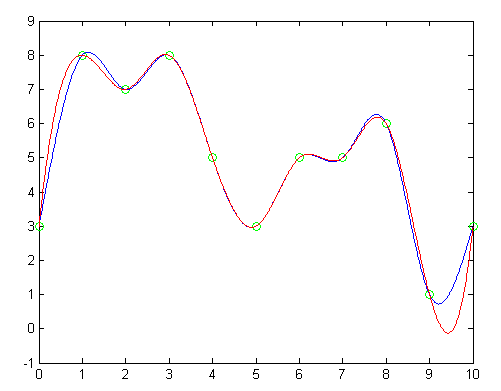
\includegraphics[width=0.5\textwidth]{spline2.png}\\
Wynik interpolacji. Zielony: funkcje wzorcowe; Czerwony: funkcja interpolująca z Matlaba; Niebieski: funkcja interpolująca z CubicSplineFast
\end{center}
	
Wynik interpolacji w Matlabie nie pokrywa się z interpolacją klasy. Różne kształty krzywych. Obie interpolacje spełniają warunek $S(x_i) = f(x_i)$.

Funkcja $f(x) = sin(x)$

Węzły $x = [-5:0.7:5]$

Interpolowana w punktach $x = [-3:0.05:3]$

\begin{center}
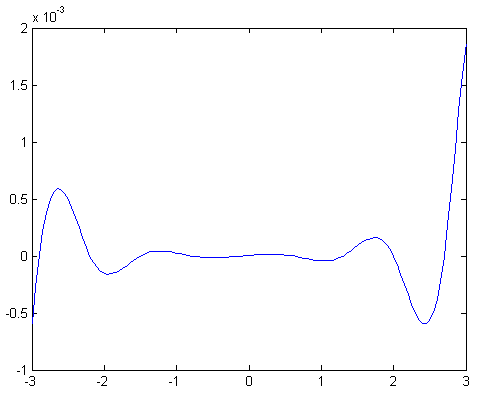
\includegraphics[width=0.5\textwidth]{spline3.png}\\
Wykres różnic
\end{center}

Wyniki interpolacji są zbliżone (największa różnica $0.0018616$, punkty przegięcia takie same). Największe różnice są na krańcach przedziałów.

Funkcja $f(x) = x^3 + x^2$

Węzły $x = [-3:0.1:5]$

Interpolowana w punktach $x = [-3:0.05:5]$

\begin{center}
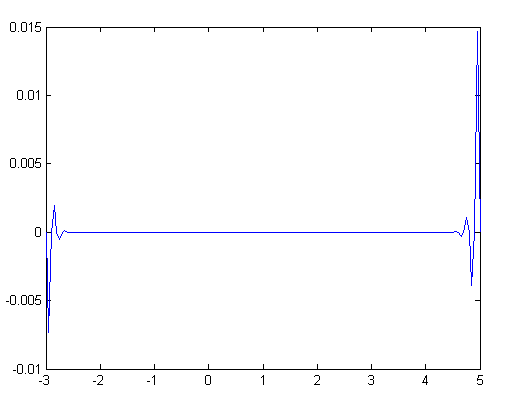
\includegraphics[width=0.5\textwidth]{spline4.png}\\
Wykres różnic
\end{center}

Wyniki interpolacji są zbliżone (największa różnica $0.014641$, punkty przegięcia takie same). Największe różnice są na krańcach przedziałów.

Funkcja $f(x) = x^-3$

Węzły $x = [2:1:2] \ 0$

Interpolowana w punktach $x = [-0.5:0.01:0.5]$

\begin{center}
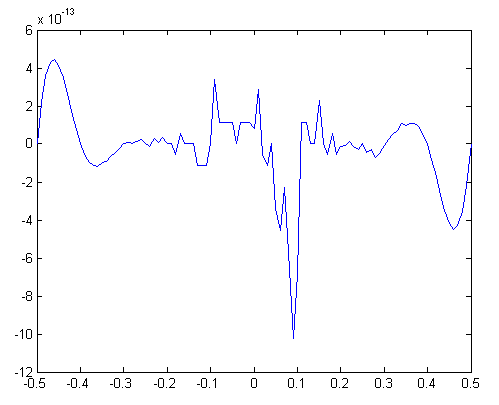
\includegraphics[width=0.5\textwidth]{spline5.png}\\
Wykres różnic
\end{center}

Wyniki interpolacji są zbliżone (największa róznica $1.0232 * 10^{-12}$, punkty przegięcia takie same).
\end{description}

\subsubsection{Testy białoskrzynkowe}
\begin{description}
\item [Opis] Metoda interpolate odpowiada za interpolację funkcjami sklejanymi 3 stopnia. Przeprowadzone zostały testy zarówno dla wartości x znajdującymi się w przedziale podanych węzłów jak i spoza zakresu. Również zostało zbadane zachowanie dla węzłów o tej samej wartości w przedziale oraz dla przedziału o krańcu będącym punktem w +nieskończoność.

\item [Sposób realizacji]

\item[ Przypadek interpolate\_InRangeTest] Jest to normalny przypadek spełniający warunki postawione przez autora klasy, czyli: wartość x należy do zakresu węzłów. W tym przypadku testowym pokrycie stanowi 93\%.\\
Pokrycie nie obejmuje wyrzucenia wyjątku będącego instrukcją gałęzi warunkowej.

\begin{lstlisting}
@Test
public void interpolate_InRangeTest() {
    xx = 2.5e-7;
    yy=cs.interpolate(xx);
    assertEquals(1.5058693318301968, yy, eps);
}
\end{lstlisting}

\item [Przypadek interpolate\_OutOfRangeTest] Jest to również normalny przypadek, mimo że wartość nie należy do zakresu wartości x. Metoda ta została okrojona z warunków sprawdzania czy podany parametr należy do przedziału, dlatego też nie ma informowania w żaden sposób użytkownika.\\
Efektem tego jest brak pokrycia instrukcji, oprócz wyrzucenia wyjątka, w gałęzi else w pętli while(ponieważ podany parametr jest mniejszy od każdego elementu zakresu).\\
Pokrycie wynosi 87\%.

\begin{lstlisting}
@Test
public void interpolate_OutOfRangeTest() {
    xx = 100e-9;
    yy=cs.interpolate(xx);
    assertEquals(1.6136430500055632, yy, eps);
}
\end{lstlisting}

\item [Przypadek interpolate\_SamePointsTest] Przypadek dla którego podane są tablice zawierające punkty o tej samej wartości. Powoduje to wychwycenie wyjątku IllegalArgumentException w gałęzi if oraz nie pokrycie gałęzi else jak i dalszej instrukcji zwracającej return. Przypadek oczekuje zwrócenia wyjątku.\\
Pokrycie instrukcji wynosi 73\%. 

\begin{lstlisting}
@Test(expected=IllegalArgumentException.class)
public void interpolate_SamePointsTest() {
    x = new double[]{0,1,1};
    y = new double[]{1,2,3};
    cs = new CubicSplineFast(x, y);
    xx = 1;
    yy=cs.interpolate(xx);
    assertEquals(1.5058693318301968, yy, eps);
}
\end{lstlisting}

\item [Przypadek interpolate\_PositiveInfTest] Oczekuje jako jednego z parametrów tablicy z wartością na końcu przedziału Double.POSITIVE\_INFINITY. Z tego względu że na końcu jest stała o wielkiej wartości, zwracana jest wartość Double.NaN(Not a Number). Również nie zostaje pokryta instrukcja if we wnętrzu której znajduje się instrukcja wyrzucenia wyjątku.\\
Pokrycie wynosi 87\%.

\begin{lstlisting}
@Test
public void interpolate_PositiveInfTest() {
    x = new double[]{0, 1, 1, 4};
    y = new double[]{1, 2, 3, Double.POSITIVE_INFINITY};
    cs = new CubicSplineFast(x, y);
    xx = 2;
    yy=cs.interpolate(xx);
    assertEquals(Double.NaN, yy, eps);
}
\end{lstlisting}

\item [Wynik] Metoda interpolate pokrywana jest w pełni jeżeli parametr należy do zakresu wartości x oraz tablice wewnętrzne obiektu są wieloelementowe z powtarzającymi się wartościami w tablicy węzłów x.
\end{description}
\section{Podsumowanie}

\subsection{Pokrycie}

Osiągnięto pełne pokrycie testowanej klasy.

\subsection{Znalezione nieprawidłowości}

Udało się doprowadzić do wygenerowania błędnych wyników.

Tworzone interpolacje często różniły się mniej lub bardziej od interpolacji generowanych przez Matlaba, jednak zawsze kształt krzywych był taki sam. Znaleziono jednak zestaw danych który powoduje wygenerowanie zupełnie innej funkcji interpolującej niż generowana przez Matlab. Można to tłumaczyć zastosowaniem innego (lepszego?) algorytmu liczenia funkcji sklejanych w Matlabie.

Znaleziono zestaw danych testowych powodujących błędne liczenie drugiej pochodnej.

\subsection{Wnioski z przeprowadzonych testów}

Stwierdzono, że klasa potrafi liczyć interpolacje funkcjami sklejanymi z pewnym przybliżeniem oraz pewną rzetelnością. Ze względu na znalezione nieprawidłowości które prawdopodobnie wynikają z zastosowanego algorytmu (nie znaleziono błędów w samej implementacji), klasa nie powinna być stosowana w produkcyjnym środowisku. Nie udało się określić klasy równoważności powodującej błędne obliczenia.

\end{document}
